\nnarticleheader{Impartial Games and the Sprague-Grundy Theorem}{Gary Gao, Haverford '21}
\noindent
\textbf{Overview -- Impartial Games}

	In combinatorics, there has been a field that studies the processes and outcomes of games -- Game Theory. And among many games, the impartial games are the most fundamental ones to study. To highlight the point of this topic, I can say that this particular section of the impartial game reveals how millions of games work, which means some generalization can provide us with many intuition and insights about game strategies.
	\begin{definition}
		An impartial game is a game in which the allowable/possible moves depend only on the position at which the game is and not on which of the players is currently moving, and where the payoffs are symmetric.
	\end{definition}
	
	In other words, the only difference between player 1 and player 2 (or other players) is that player 1 goes first. The game is played until a terminal position is reached, in which an additional move is not possible. Then one of the players is declared the winner and the other the loser. Furthermore, in order to fully understand the strategies of the game, impartial games are played with perfect information and no chance moves, meaning all information about the game and operations for both players are visible to both players, and all players play their best possible moves usually. \textbf{Our goal is to determine what are the best or the most favorable strategies for each player at each position of the game.} More specifically, which player has the winning strategy at the moment if the game proceeds to a certain situation? Or if the game can be forced to a draw?

\noindent
\textbf{The Nim Game}

\noindent
\textbf{An Intuitive Example}

Here is a famous and simple game:
		\begin{problem}
			There is a pile of 100 stones on the ground. Two players, called Alice and Bob, play the following game: Starting with Alice, each player can and must take away 1, 2, or 3 stones. At the end, the player who takes away the last stone wins. Who has the winning strategy? And what is his/her strategy?
		\end{problem}
		\begin{solution}
			The strategy is not hard to spot. We can see that there is a nice way for Bob to counter a move made by Alice. Since one can only take 1,2, or 3 stones, it reminds us that we can utilize the divisibility of 4. Whenever Alice takes $n$ stones away, bob can then take $(4-n)$ away so that after a round, the number of stones left is still divisible by 4 (since $4|100$). Therefore, Bob can secure the last stone since his move would always be reducing the number of stones to a multiple of 4.
		\end{solution}
	
	\noindent
	\textbf{What Is A Nim Game?}
	
		\begin{definition}
		A Nim game is a game in which two players take turns removing objects from distinct piles. During each move a player must remove at least one object, and the player can remove any number of objects from the same pile. 
		\end{definition}
		
		We can see that a definition for the most general Nim game is similar to the example we touched on earlier. But the key element here is that one player can remove \textbf{any} amount of objects from a pile. Now there is a question: what is the point of the game if all stones may be removed at once? The answers is: yes, the game with only 1 pile is trivial now. But what if we have multiple piles?
		\begin{problem}
			There are two piles of stones. The first one has $a$ stones and the second one has$b$. Alice and Bob plays the Nim game on these two piles starting with Alice. Who has the winning strategy, and why?
		\end{problem}
		To fully understand the mechanism and lay a foundation for further exploration, we now introduce a method.
	
\noindent	
	\textbf{Winning And Losing Positions}
	
		To simplify the problems, we consider that the game has a winning-losing outcome for sure.
		\begin{definition}
			A winning position is a position of the game at which the player making the subsequent move has a winning strategy. A losing position is a position of the game at which the player making the subsequent move will not have any strategy to win, which means that (one of) the player's opponents has a winning strategy.
		\end{definition}
		Now we try to find some nice properties about the game when there are 2 players.
		\begin{theorem}
			In a game with 2 players, a position is winning if and only if the player making a move can change the situation to a losing position after he moves.
		\end{theorem}
		This is obvious. If player 1 changes the game to a losing position, then player 2 will definitely lose (so that player 1 wins), making the original position a winning position. In all the following explanations and solutions to the problems we refer ``winning" and ``losing" positions as winning or losing for Player 1. And a winning position is denoted by ``$+$" and a losing one by ``$–$" for simplicity.
		
\noindent
	\textbf{Solution to 2 Pile Nim Games}
	
		\begin{solution}
			Denote $(a,b)$ as the case where the two starting piles have $a$ and $b$ stones respectively.\\
			\indent First notice that by an extension of the definition $(0,0)$ is a losing position because before this step Bob already won. Therefore, we use the following method to fill out a table: place $(0,0)$ at the top left. As $a$ or $b$ increases, we put a ``-" in the cell $(a,b)$ if and only if there is no other ``-" signs to the left or top of the cell.
			\begin{center}
			\begin{tabular}{|c|c|c|c|c|c|c|}
			\hline
			$(a,b)$&0&1&2&3&4&...\\
			\hline
			0&-&+&+&+&+&...\\
			\hline
			1&+&-&+&+&+&...\\
			\hline
			2&+&+&-&+&+&...\\
			\hline
			3&+&+&+&-&+&...\\
			\hline
			4&+&+&+&+&-&...\\
			\hline
			...&...&...&...&...&...&...\\
			\hline
			\end{tabular}
			\end{center}
			
			Then we can clearly see that it is a losing position for Alice if and only if the two starting piles have the same amount of stones. We can verify and prove this in two ways. One is by some simple induction. The other one is that whenever Alice removed some stone in pile 1, Bob imitates that move in pile 2 so that he can secure the victory.
		\end{solution}
		\noindent
	\textbf{Solution to The General Nim Game}
	
		\begin{problem}
			There are $n$ piles of stones. The $k$th pile has $a_k$ stones ($1\leq k\leq n$). Alice and Bob plays the Nim game on these n piles starting with Alice. Who has the winning strategy, and why?
		\end{problem}
		We can first try to explore with the case where $n=3$. By filling out some tables with different $(a_1,a_2,a_3)$, we can certainly find some patterns but they do not appear in a nice way. We can try to obtain a pattern via brute force through all triplets of numbers of stones but the pattern do not have any apparent recursion. (It is also hard because the table would be 3-dimensional). However, it is possible for us to see that in most cases, Alice will still win. We can also obtain some small cases where the starting position is a losing one for Alice:\\
		WLOG, organize them in the way that $a_1 \leq a_2 \leq a_3$
		\begin{center}
		$(0,1,1),(0,2,2),(0,3,3),...$\\
		$(1,2,3),(1,4,5),(1,5,6),...$\\
		$(2,4,6),(2,5,7),(2,8,10),(2,9,11),(2,12,14)...$\\
		$(3,4,7),(3,5,6),(3,8,11),(3,9,10),(3,12,15)...$\\
		$(4,8,12),(4,9,13),(4,10,14),(4,11,15),(4,16,20),...$\\
		\end{center} 
		Using intuition, we can begin to see that the triplets have some characteristics of cycles of 1,2,4,..., the powers of 2. Thus, we explore them in a way related to binary expressions of integers.\\
		\begin{definition}
			Nim Plus $a \oplus b$ for integers $a,b$ is defined as the bitwise exclusive or operation on the binary expressions of the number $a$ and $b$.
		\end{definition}
		The exclusive or operation means that $1 \oplus 1 = 0 \oplus 0 = 0, 1 \oplus 0 + 0 \oplus 1 = 1$. We do this operation on every digit of the binary expression of 2 numbers independently and combine them together. For example, $113=(1110001)_2, 189=(10111101)_2$
	
		\begin{center}
			\begin{tabular}{ccccccccc} 
			&1&0&1&1&1&1&0&1\\
			$\oplus$&&1&1&1&0&0&0&1\\
			\hline
			&1&1&0&0&1&1&0&0
		\end{tabular}
		\end{center}
		So $113 \oplus 189 = (11001100)_2 = 204$. Also notice that the Nim sum obey the associative and the commutative laws, and that $x \oplus y = 0$ if and only if $x = y$.
		\begin{theorem} 
		In a Nim game using $n$ piles with $a_1, a_2, a_3, ... , a_n$ stones in the 1st, 2nd, 3rd, ..., nth pile respectively, the starting position is a losing one for the first player if and only if $a_1 \oplus a_2 \oplus a_3 \oplus...\oplus a_n$ = 0.			
		\end{theorem}
		\begin{proof}
		Let a situation be $X = (x_1,x_2,...,x_n)$. Let a situation after doing one move on $X$ be $Y = (y_1,y_2,...,y_n)$. Let $p = x_1 \oplus x_2 \oplus... \oplus x_n$, $ q = y_1 \oplus y_2 \oplus ... \oplus y_n$. Let $x_k$ and $y_k$ be the number of stones in the $k$th pile (the one that is changed) before and after the move.  By definition $x_i = y_i$ except when $i=k$. Therefore:
		\begin{align}
		\nonumber q &= y_1 \oplus y_2 \oplus ... \oplus y_k \oplus ... \oplus y_n\\
		\nonumber   &= x_1 \oplus x_2 \oplus ... \oplus x_{k-1} \oplus y_k \oplus ... \oplus x_n\\
		\nonumber   &= x_1 \oplus x_2 \oplus ... \oplus x_{k-1} \oplus y_k \oplus (x_k \oplus x_k) \oplus ... \oplus x_n\\
		\nonumber   &= x_1 \oplus x_2 \oplus ... \oplus x_k \oplus ... \oplus x_n \oplus x_k \oplus y_k\\
		\nonumber   &= p \oplus x_k \oplus y_k
		\end{align}
		
		\indent We first prove that if $p=0$ then after a move $q\neq0$. If $p=0$, $q=x_k \oplus y_k$, which cannot be zero because $x_k \neq y_k$.\\
		\indent Then, if $p\neq0$, we prove that there exist some number $a \leq \max\{x_1,x_2,...,x_n\}$ such that for some $x_k \leq a$, $q = p \oplus x_k \oplus a = 0$ (which means we reduce the kth pile to $a$ stones). In fact, if we let $a = x_1 \oplus x_2 \oplus ... \oplus x_{k-1} \oplus x_{k+1} \oplus ... \oplus x_n$, it satisfies the condition that $q = 0$. We just have to prove that it is possible for us to find a $k$ such that $x_1 \oplus x_2 \oplus ... \oplus x_{k-1} \oplus x_{k+1} \oplus ... \oplus x_n \leq x_k$. Notice that this $a$ is equivalent to $p \oplus x_k$. Let's find the leftmost nonzero digit of the binary representation of $a$ to be the $d$th digit from the right. Then, there must exist a $x_k (1\leq k\leq n)$ such that its $dth$ digit from the right is nonzero (which mean it is 1). This is because if all of the $x_i$ have zero on that digit, $a$ must be zero, making a contradiction.\\
		\indent Therefore, we've established that if $p=0$ then $q\neq0$ and vice versa, establishing a connection between two types of positions. Since empty piles are defined to be losing for the first player, we can easily see by induction that the theorem is proved.
		\end{proof}
		Thus ends our solution to the problem of Nim Games.

\noindent
\textbf{The Sprague-Grundy Theorem}

\noindent
	\textbf{History}
	
		The Sprague-Grundy theorem and its proof contains the main results of a theory discovered independently by German Mathematician Roland. P. Sprague (1935) and English Mathematician Patrick. M. Grundy (1939). Therefore the theorem is named after both of them.
		
		\noindent
	\textbf{Theorem Statement}
		\begin{theorem}
			\textbf{Sprague-Grundy Theorem:} Every impartial game under the normal play convention is equivalent to a nimber (which is a Nim Game with 1 single pile).
		\end{theorem}
		The normal play convention here refer to the common and standard ways to determine a game's winner; e.g. \textbf{preventing the other player from being able to move}, being the first player to achieve a target, having the highest value of something, etc. Therefore, in our case, the theorem states that every impartial game is just equivalent to the Nim game we just solved. The proof of the theorem is very complicated and abstract thus it would not be given explicitly here. Intuitively, the proof uses induction to classify every possible position of the game by assigning it a number $a$, indicating that the position is equivalent to a pile of $a$ stones in a Nim Game. Then it is also possible to show that the Nim Game is the \textbf{same} even if you allow arbitrary \textbf{adding of stones} to a pile as a possible move (as long as there are some limitations to ensure that the number of stones will reduce to zero). For instance, if a situation can go to situations that correspond to 1,2,3,... stones in a pile after a move, the situation will be equivalent to a 0-pile (the losing position for the first player by definition). 
		\noindent
	\textbf{Remarks}
	
		 Although the theorem does not provide any specific way to map the equivalence or conversion, it still offers some very helpful insights in solving these problems. Basically, when we encounter any impartial game, we can try to convert it to a Nim Game. 
		 \noindent
	\textbf{An Example}
	
		\begin{problem}
			Suppose we have a chocolate bar composed of small squares of chocolate that form a triangle. There is a square with bad taste somewhere in the middle. Alice and Bob alternate to cut off and eat a rectangular piece along the horizontal/vertical grid (only one straight cut allowed each time) that does not contain the bad square. Who has the strategy to force the other player to eat the bad square finally?
		\end{problem}
	
		\begin{solution}
			With the idea of Sprague-Grundy theorem, we can try to come up with a nice way to link the actual game to some Nim Game. Such a construction can be found with the help of a diagram (red cell indicating the bad square):\\

\begin{figure}[h]
  \begin{center}
    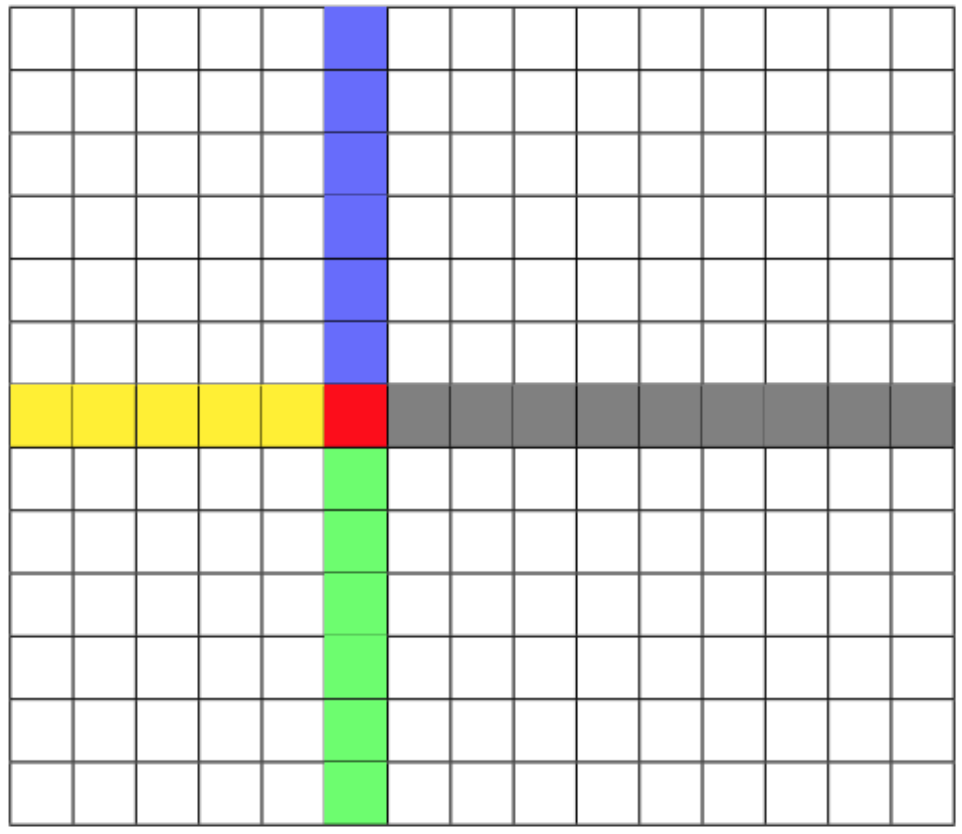
\includegraphics[scale=.6]{gao_diagram}
  \end{center}
\end{figure}

			\indent Then we can see that each move is equivalent reducing one of the four strips (blue, gray, yellow, and green) to any nonnegative amount of squares by making one horizontal/vertical cut. This game is exactly the same with a Nim Game with 4 piles. Therefore, if the four strips have $x_1,x_2,x_3,x_4$ squares respectively, Bob will win if and only if $x_1 \oplus x_2 \oplus x_3 \oplus x_4 = 0$.
		\end{solution}
		\noindent
	\textbf{Summary}
	
		The study of impartial games contributes to the combinatorial game theory field and broadens our understanding in all sorts of non-impartial games that humans have created (chess, checkers, pokers, etc) as well. We can see that the buildup to Sprague-Grundy theorem is relatively long, since solving the Nim Game completely requires some new lemmas and definitions. The formulation of the theorem is concise but also links all impartial games together, which shows most charming element of combinatorics: It is a study dedicating to the conversion very broad, abstract, and verbal problems and objects to organized, rigorous, and powerful results and theorems in mathematics.